\documentclass[11pt]{article}

% ============================================================
%  A verification pearl from Dempwolff--Mueller
%  "Permutation polynomials and translation planes of even
%   order", Adv. Geom. 13 (2013).
%  Style: minimal words, many pictures.  Companion to pearl.lean
% ============================================================

\usepackage[a4paper,margin=17mm]{geometry}
\usepackage{amsmath,amssymb}
\usepackage{tikz}
\usepackage{tikz-cd}
\usepackage{xcolor}
\usepackage{parskip}
\usetikzlibrary{arrows.meta,positioning,calc,decorations.pathmorphing,
  decorations.markings,shapes.geometric,shapes.misc,backgrounds,fit,
  graphs,quotes,patterns,matrix,chains,angles}

% ---- palette (matches patterns.tex) --------------------------
\definecolor{cA}{HTML}{1b4965}
\definecolor{cB}{HTML}{5fa8d3}
\definecolor{cC}{HTML}{cae9ff}
\definecolor{cD}{HTML}{e07a5f}
\definecolor{cE}{HTML}{81b29a}
\definecolor{cF}{HTML}{f2cc8f}
\definecolor{cG}{HTML}{6a4c93}
\definecolor{ink}{HTML}{22223b}

\tikzset{
  dot/.style={circle,fill=cA,inner sep=1.5pt},
  odot/.style={circle,draw=cA,fill=white,inner sep=1.5pt},
  box/.style={rounded corners=2pt,draw=cA,thick,fill=cC,inner sep=4pt,align=center},
  chip/.style={rounded corners=3pt,draw=cA,very thick,fill=cF,inner sep=5pt,align=center,font=\small},
  hit/.style={rounded corners=2pt,draw=cA,very thick,fill=cE,inner sep=3pt,align=center,font=\small\bfseries},
  miss/.style={rounded corners=2pt,draw=cB,fill=white,inner sep=3pt,align=center,font=\scriptsize,text=cB},
  maparrow/.style={-{Stealth[length=3mm]},thick,cA},
  bij/.style={<->,{Stealth[length=2.6mm]}-{Stealth[length=2.6mm]},thick,cD},
}

\newcommand{\GF}[1]{\mathrm{GF}(#1)}
\newcommand{\heading}[1]{%
  \begin{center}\begin{tikzpicture}
    \node[fill=cA,text=white,rounded corners=3pt,inner xsep=8pt,inner ysep=4pt,
      font=\large\bfseries]{#1};
  \end{tikzpicture}\end{center}\vspace{-1mm}}

\pagestyle{empty}

\begin{document}

% =============================================================
% TITLE
% =============================================================
\begin{center}
{\LARGE\bfseries\color{cA} A Verification Pearl}\\[2mm]
{\large\color{ink} The two Dempwolff--M\"uller polynomials are the \emph{only} ones,\\
in the smallest field}\\[3mm]
{\small A one-page, fully machine-checked classification in Lean 4.\quad Companion file: \texttt{pearl.lean}}
\end{center}

\vspace{2mm}

% ---- the pearl in a box -------------------------------------
\begin{center}
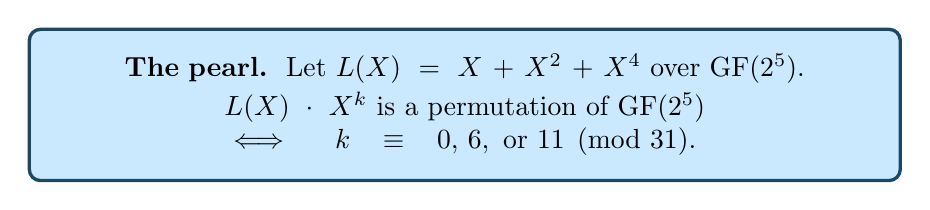
\begin{tikzpicture}
\node[draw=cA,very thick,rounded corners=4pt,fill=cC,inner sep=9pt,align=center,text width=0.86\linewidth]{%
  \bfseries The pearl.\normalfont\ \ Let $L(X)=X+X^2+X^4$ over $\GF{2^5}$.\\[2pt]
  $L(X)\cdot X^{k}$ is a permutation of $\GF{2^5}$\ \ $\iff$\ \ $k\equiv 0,\,6,\text{ or }11\pmod{31}$.};
\end{tikzpicture}
\end{center}

\vspace{1mm}
\noindent
The paper builds permutation polynomials $L(X)\cdot X^{k}$ over $\GF{2^n}$.
For the smallest interesting case ($n=5$, $m=3$) we \emph{classify all of them}:
apart from the trivial $k=0$, the exponents are exactly the paper's $k$ and its
companion $k'$. Nothing else works.

% =============================================================
\heading{1.\ \ The field $\GF{2^5}$: a clock of 31}
% =============================================================
\begin{center}
\textit{Nonzero elements $=$ powers of a generator $g$. Order $31$ (prime).}
\end{center}
\begin{center}
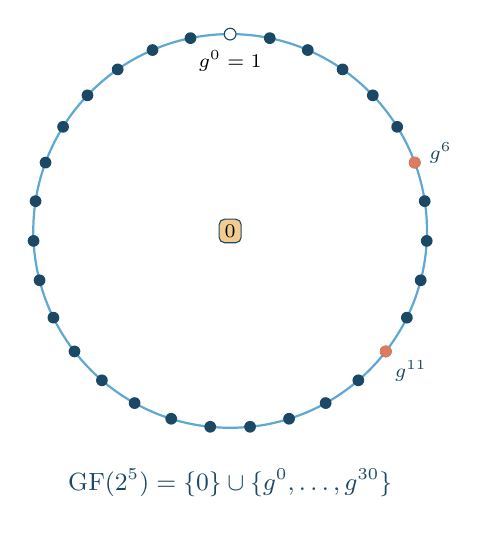
\begin{tikzpicture}[scale=1]
  \def\R{2.5}
  \draw[cB,thick] (0,0) circle (\R);
  \foreach \i in {0,...,30}{
    \node[dot] (n\i) at ({90-\i*360/31}:\R){};
  }
  \node[odot,label={[font=\scriptsize]below:$g^{0}=1$}] at (90:\R){};
  \node[font=\scriptsize,cA] at (90-6*360/31:\R+0.35) {$g^{6}$};
  \node[font=\scriptsize,cA] at (90-11*360/31:\R+0.4) {$g^{11}$};
  \node[dot,fill=cD] at (90-6*360/31:\R){};
  \node[dot,fill=cD] at (90-11*360/31:\R){};
  \node[rectangle,draw=cA,fill=cF,rounded corners=2pt,inner sep=2pt,font=\scriptsize] at (0,0){$0$};
  \node[font=\small,cA] at (0,-\R-0.7){$\GF{2^5}=\{0\}\cup\{g^0,\dots,g^{30}\}$};
\end{tikzpicture}
\end{center}
\begin{center}
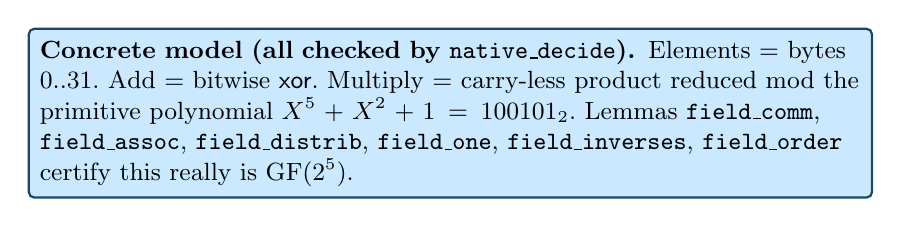
\begin{tikzpicture}
\node[box,text width=0.86\linewidth,align=left,font=\small]{%
  \textbf{Concrete model (all checked by \texttt{native\_decide}).}
  Elements $=$ bytes $0..31$.\ Add $=$ bitwise \textsf{xor}.\
  Multiply $=$ carry-less product reduced mod the primitive polynomial
  $X^5+X^2+1=100101_2$.\ Lemmas \texttt{field\_comm}, \texttt{field\_assoc},
  \texttt{field\_distrib}, \texttt{field\_one}, \texttt{field\_inverses},
  \texttt{field\_order} certify this really is $\GF{2^5}$.};
\end{tikzpicture}
\end{center}

% =============================================================
\heading{2.\ \ Two easy bijections, one hard product}
% =============================================================
\begin{center}
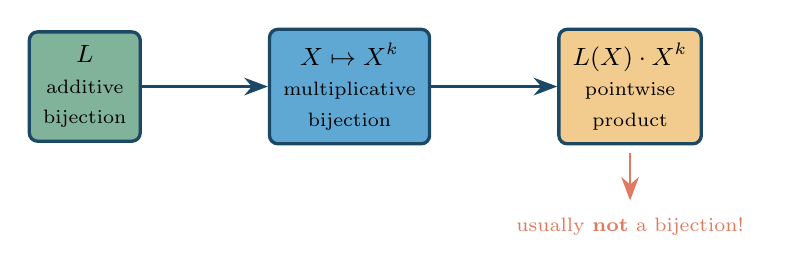
\begin{tikzpicture}[node distance=6mm]
  % additive box
  \node[chip,fill=cE] (add) {$L$\\ \scriptsize additive\\ \scriptsize bijection};
  \node[right=16mm of add,chip,fill=cB] (mul) {$X\mapsto X^{k}$\\ \scriptsize multiplicative\\ \scriptsize bijection};
  \node[right=16mm of mul,chip,fill=cF] (prod) {$L(X)\cdot X^{k}$\\ \scriptsize pointwise\\ \scriptsize product};
  \draw[maparrow] (add.east)--(mul.west);
  \draw[maparrow] (mul.east)--(prod.west);
  \node[below=8mm of prod,text width=3.2cm,align=center,font=\scriptsize,text=cD]
    {usually \textbf{not} a bijection!};
  \draw[maparrow,cD] ($(prod.south)+(0,-1mm)$) -- ++(0,-6mm);
\end{tikzpicture}
\end{center}
\begin{center}\small
$L$ is a permutation; each $X^{k}$ ($k=1..30$) is a permutation.
But the pointwise product of two permutations is \emph{rarely} a permutation.
\end{center}

% =============================================================
\heading{3.\ \ The classification: only 3 exponents survive}
% =============================================================
\begin{center}
\textit{Is $L(X)\cdot X^{k}$ a permutation? \ \ (green $=$ yes)}
\end{center}
\begin{center}
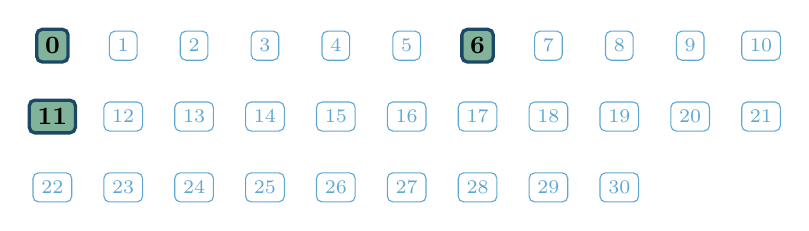
\begin{tikzpicture}[x=0.9cm,y=0.9cm]
  \foreach \k in {0,...,30}{
    \pgfmathtruncatemacro{\col}{mod(\k,11)}
    \pgfmathtruncatemacro{\row}{-div(\k,11)}
    \ifnum\k=0 \node[hit] at (\col,\row){0}; \else
      \ifnum\k=6 \node[hit] at (\col,\row){6}; \else
        \ifnum\k=11 \node[hit] at (\col,\row){11}; \else
          \node[miss] at (\col,\row){\k};
    \fi\fi\fi
  }
\end{tikzpicture}
\end{center}
\begin{center}\small
Out of the $30$ permutation monomials, exactly $\{6,11\}$ keep the product a
permutation. Verified exhaustively: \ \texttt{dm\_classification}, \ \texttt{dm\_rarity}.
\end{center}

% =============================================================
\heading{4.\ \ What the three winners are}
% =============================================================
\begin{center}
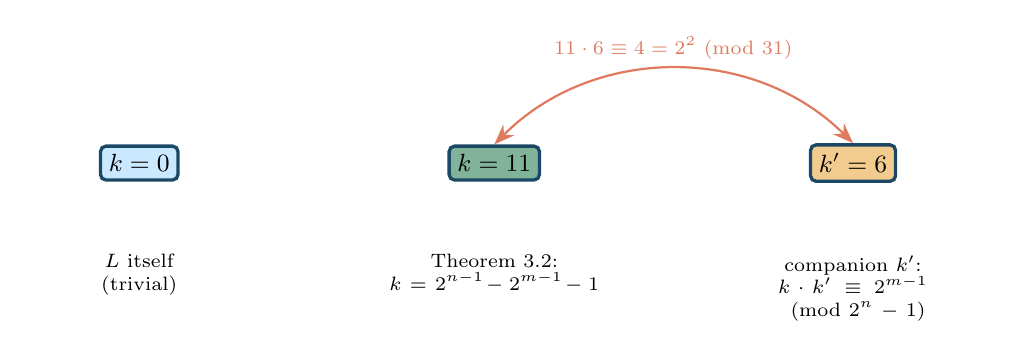
\begin{tikzpicture}[node distance=5mm]
  \node[hit,fill=cC] (k0) {$k=0$};
  \node[right=34mm of k0,hit,fill=cE] (k11) {$k=11$};
  \node[right=34mm of k11,hit,fill=cF] (k6) {$k'=6$};
  \node[below=8mm of k0,font=\scriptsize,align=center,text width=2.6cm]{$L$ itself\\(trivial)};
  \node[below=8mm of k11,font=\scriptsize,align=center,text width=3.0cm]
    {Theorem 3.2:\\ $k=2^{n-1}\!-2^{m-1}\!-1$};
  \node[below=8mm of k6,font=\scriptsize,align=center,text width=3.0cm]
    {companion $k'$:\\ $k\cdot k'\equiv 2^{m-1}$\\ $\pmod{2^n-1}$};
  % relation arc
  \draw[bij] (k11.north) to[bend left=45] node[above,font=\scriptsize,text=cD]{$11\cdot 6\equiv 4=2^{2}\ (\mathrm{mod}\ 31)$} (k6.north);
\end{tikzpicture}
\end{center}
\begin{center}\small
So the paper's two constructions ($k$ and $k'$) are, for this field, the whole story.\\
Checked: \ \texttt{dm\_paper\_k}, \ \texttt{dm\_paper\_k'}, \ \texttt{kk'\_relation}, \ \texttt{mono11\_perm}.
\end{center}

% =============================================================
\heading{5.\ \ Machine-checked}
% =============================================================
\begin{center}
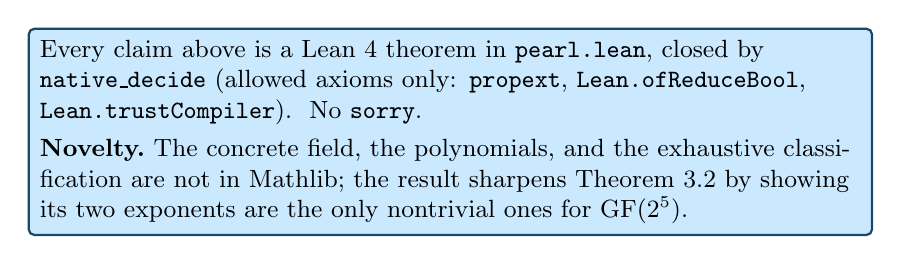
\begin{tikzpicture}
\node[box,text width=0.86\linewidth,align=left,font=\small]{%
  Every claim above is a Lean~4 theorem in \texttt{pearl.lean}, closed by
  \texttt{native\_decide} (allowed axioms only: \texttt{propext},
  \texttt{Lean.ofReduceBool}, \texttt{Lean.trustCompiler}).\ \
  No \texttt{sorry}.\\[3pt]
  \textbf{Novelty.}\ The concrete field, the polynomials, and the exhaustive
  classification are not in Mathlib; the result sharpens Theorem~3.2 by showing
  its two exponents are the only nontrivial ones for $\GF{2^5}$.};
\end{tikzpicture}
\end{center}

\vfill
\begin{center}\scriptsize\color{ink}
Source: U.\ Dempwolff and P.\ M\"uller, \emph{Permutation polynomials and translation planes of even order},
Adv.\ Geom.\ 13 (2013), 293--313.\quad Formalisation: \texttt{RequestProject/DempwolffMueller/Pearl.lean}.
\end{center}

\end{document}
